% !TEX root = ../paper.tex
\section{Discussion}

% noisy data, and binary classification
Our training data contains much variability because there are disagreements between our judgment of ``usefulness,'' rendering our results unclear.
These samples cannot be classified as either useful or not useful.
This impacts the trade-off between the precision and recall for our model, and consequently, the F$_1$ score.

% tuning the F score for precision and recall
Depending on the use case, we can fine-tune the F-score to give more weight to recall or precision.
For instance, if we wanted to measure the amount of useful comments within a large dataset, we can give more weight to precision, sacrificing some good comments.
If we wanted to modify a code review software such that it displays useful comments more prominently, we can give more weight to recall.
%\subsection{Reasons of Classification}
% reasons for classification as useful or not useful
During the training process, reasons for the judgment are recorded. Examples of reasons for positive comments include:

\begin{itemize}
	\item they contain new information;
	\item they contain constructive suggestions;
	\item they discuss directly about the change; and
	\item they discuss technical matters.
\end{itemize}

Examples of reasons for negative comments include:

\begin{itemize}
	\item chatting (i.e. no new information, just communication);
	\item not discussing directly about the change;
	\item discussing about the process workflow; and
	\item discussing about Git or Gerrit itself.
\end{itemize}



%\subsection{Binary Classification}

By removing the samples with scores of 1 and 2 from our data set, leaving with 209 samples without disagreements, we can perform a binary classification, in which all comments will receive either a positive or negative score.
By cross-validation using only samples in total agreement, we obtained a much better F$_1$ score of 0.896.

We could not objectively measure the F$_1$ score for all samples, because giving positive or negative classification to 1 and 2-scored samples introduces a bias.
However, the results seen in Fig.\ref{fig:binary} suggests that the binary classifier tends to gives positive classification to samples with score of 2 more than samples with score of 1, and the \emph{vice versa} for negative classification.

\begin{figure}[h]
\centering
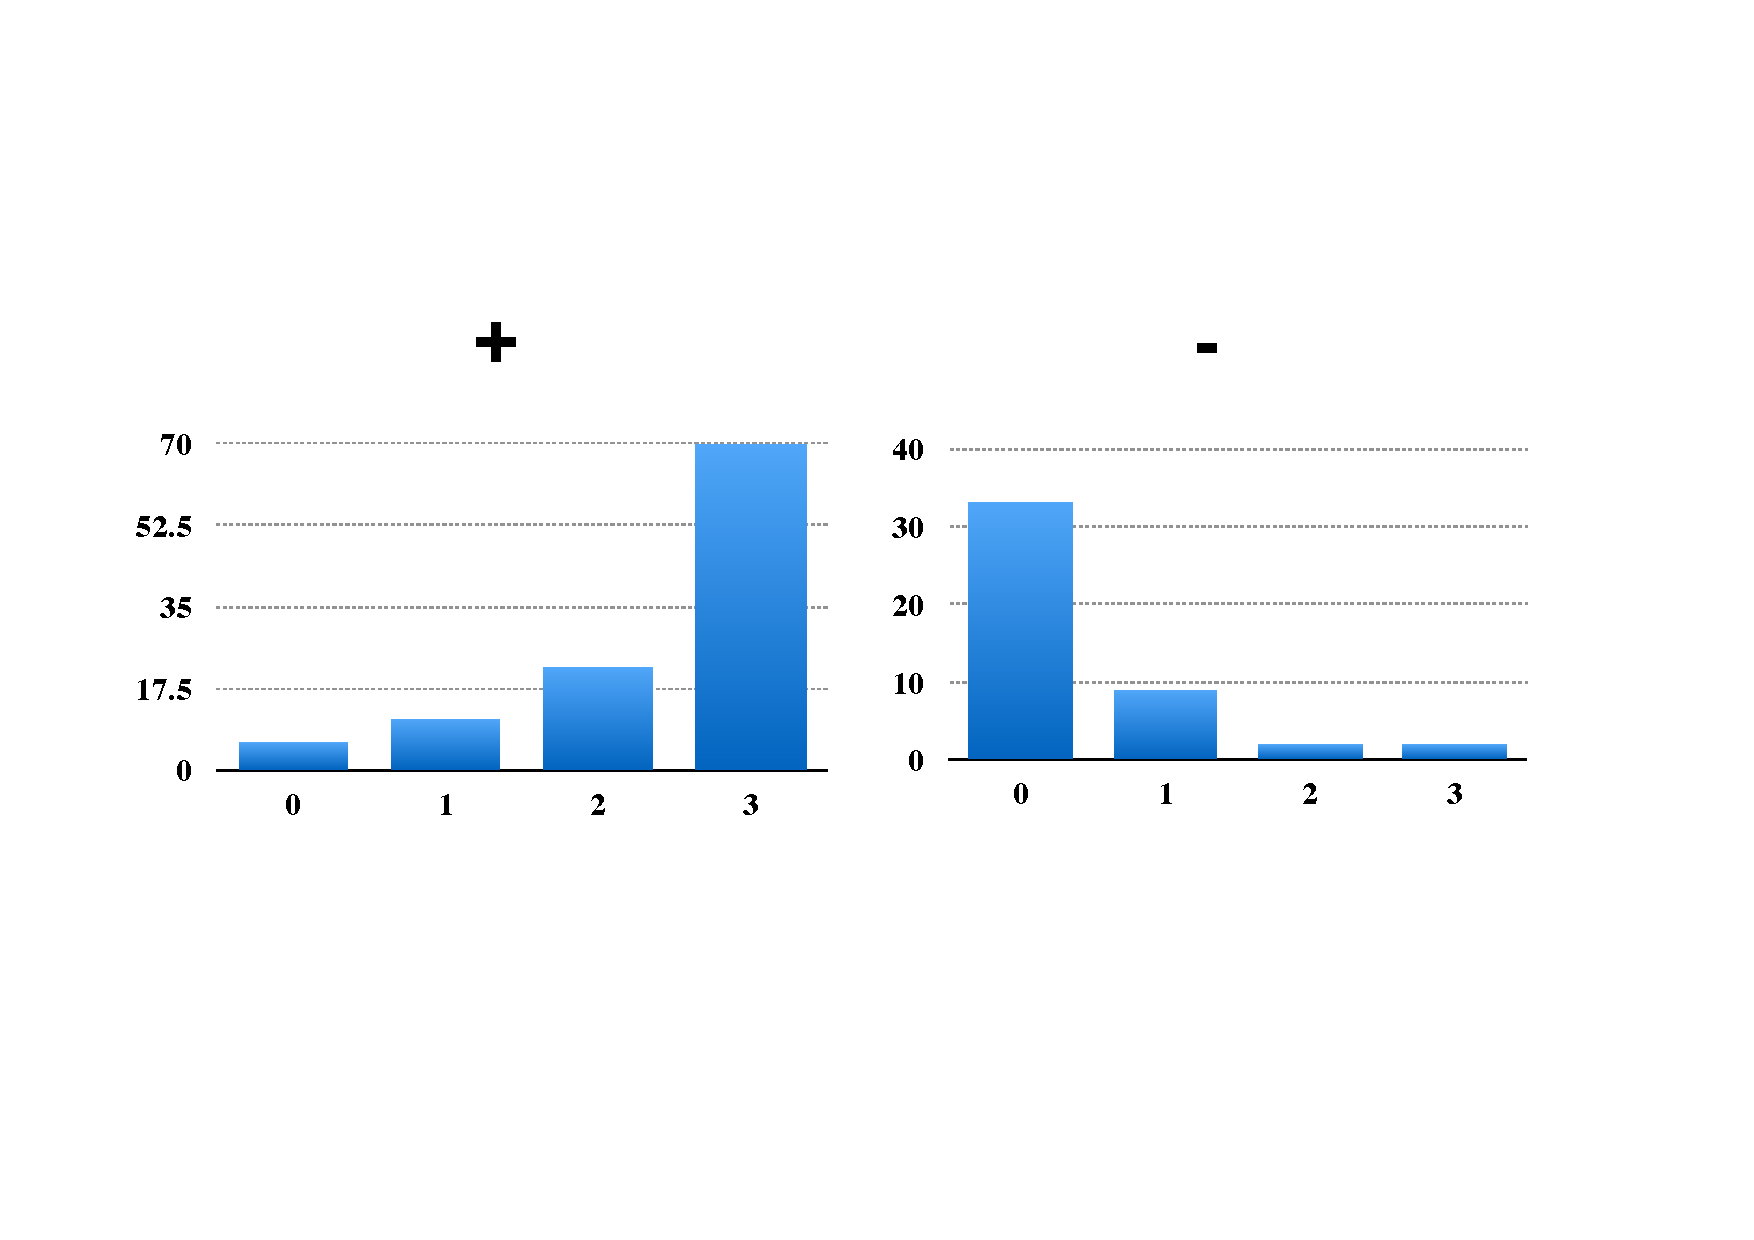
\includegraphics[width=3in]{binary}
\caption{The amount of comments by score classified by the binary classifier.}
\label{fig:binary}
\end{figure}
